\begingroup
\renewcommand\thechapter{A}
\titleformat{\chapter}[display]
{\normalfont\huge\bfseries}{}{20pt}{\Huge}
\setcounter{section}{0}
\setcounter{figure}{0} 

\chapter*{Appendix A - MongoDB installation}
\addcontentsline{toc}{chapter}{Appendix A - MongoDB installation}

MongoDB is used widely across industry, and as such, there are many versions of the software available. 
This project made use of the Community Server, a free download with most of MongoDB's key features. An alternative 
option would have been the Enterprise version, which is widely used across industry and requires users to sign 
up with a business account. In an actual production environment, the Enterprise version of the MongoDB server 
would be more beneficial due to its additional features including an in-memory storage engine as well as enhanced 
security options \autocite{mongodb_mongodb_nodate}, though the Community version still includes the necessary 
core functionality of MongoDB.

\para The community version was downloaded from the \href{https://www.mongodb.com/try/download/community}{official MongoDB website} \autocite{mongodb_try_nodate},
using the appropriate installer for a 64-bit Windows 10 system as depicted in Figure \ref{fig:MongoDownload}. Both ZIP and MSI options
are available, with the MSI being used in this project for simplicity.

\begin{figure}[H]
    \centering
    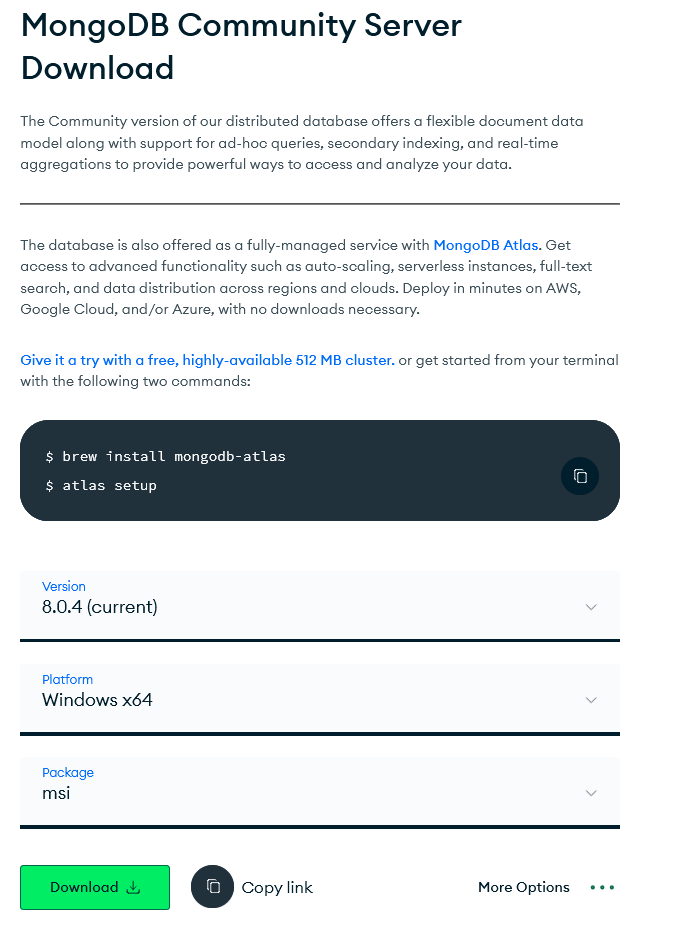
\includegraphics[width=.63\textwidth]{Mongo/Installation/MongoDB Community Site.png}
    \caption{The MongoDB Community Server download page.\label{fig:MongoDownload}}
\end{figure}

\noindent With the community server installed, a method to interface with MongoDB such as the official 
MongoDB shell is necessary, which is available from the same download page.

\begin{figure}[H]
    \centering
    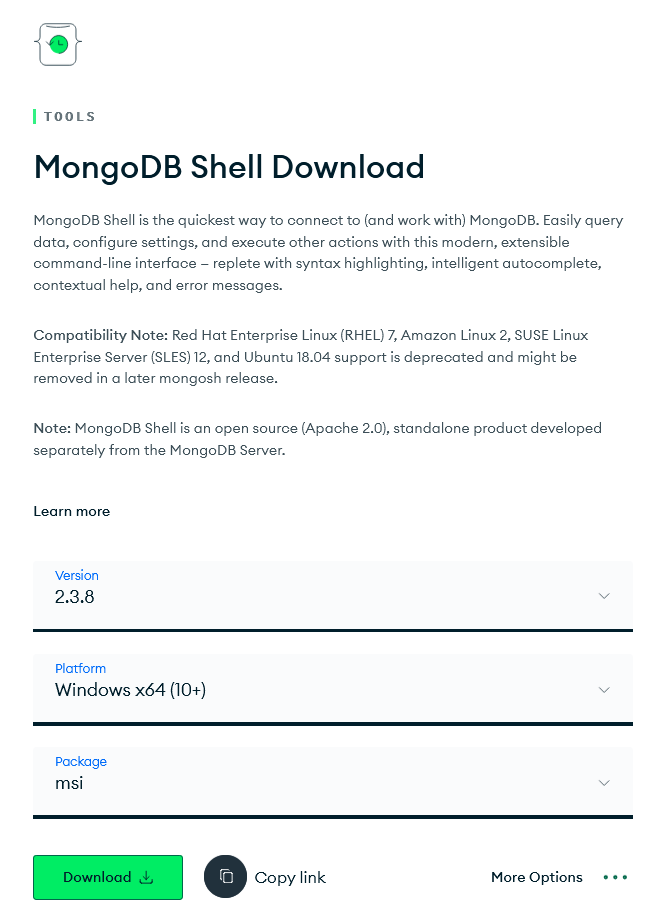
\includegraphics[width=0.5\textwidth]{Mongo/Installation/MongoDB Shell.png}
    \caption{The MongoDB Shell download page.\label{fig:MongoShellDownload}}
\end{figure}

% Talk about adding it to PATH?

\noindent The MongoDB shell allows for direct connections to MongoDB, from which commands can be run. For example, Figure \ref{fig:ShowDBs} 
depicts the "show dbs" command, which lists all databases. From a fresh install, there are three databases stored in MongoDB,
which all store meta information about the software itself.

\begin{figure}[H]
    \centering
    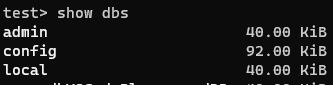
\includegraphics[width=0.5\textwidth]{Mongo/Installation/Show DBs.png}
    \caption{The results of the "show dbs" command in the MongoDB shell.\label{fig:ShowDBs}}
\end{figure}


% This maybe doesn't actually have to be an appendix, though I wasn't sure where would be best to address this topic.
% Consider that it also doesn't really need addressing at all unless you use a hyper-specific feature.

\endgroup